\subsection{Scenario 2: 2-domain topology with simple group mobility}
\label{sec:case2}

\begin{figure}[htb!] 
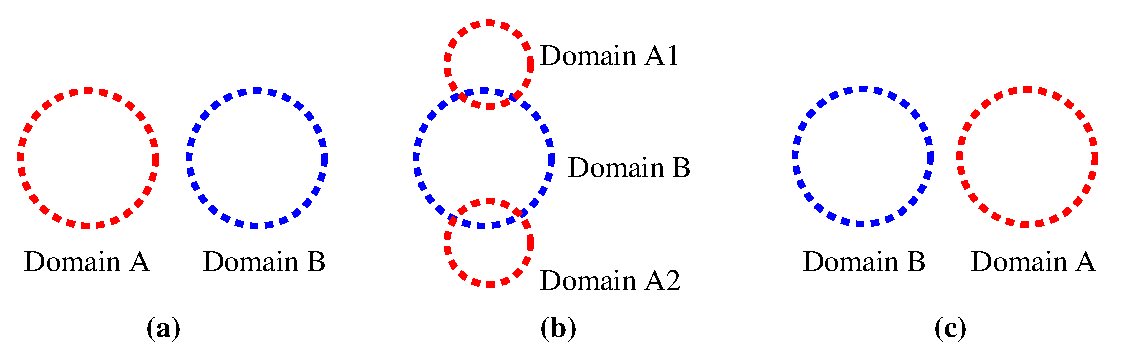
\includegraphics[width=0.47\textwidth]{figs/case2topo.eps}
\caption{Relative position of domain A and B at (a) Initial, (b) domain $A$
is partitioned, and (c) domain $A1$ and $A2$ are merged}
\label{fig:case2topo} 
\end{figure}

%we demostrate the changes of end-to-end
%performance with a simple scenario setting. 
%More detail study of random scenario will be shown in section \ref{sec:case3}.   
In this section, 
we study the performance of a simple group mobililty with 
2-domain topology shown in figure \ref{fig:case2topo}.
There are two domains in this scenario, namely domain $A$ and domain $B$. 
We create a synthetic group mobility for domain $A$ as follow: 
1) Initially, domain $A$ is located at the west side of domain $B$, 
2) After a while, domain $A$ is moving towards the east side of domain $B$ and
partitioned into two sub-domains $A1$ and $A2$,
3) Finally, $A1$ and $A2$ are merged back to domain $A$ and domain $A$ is
located at the east side of domain $B$. 
Two UDP traffics, $U1$ and $U2$, are created for the evaluation.
$U1$ is a traffic where the source is located in domain $A1$ and the destination
is located at domain $A2$. 
During domain $A$ is partitioned, $U1$ need to use the
path $A1\to B\to A2$ to maintain connectivity.
For $U2$, the source is located at domain $A$ and the destination is located at
domain $B$.

